\documentclass[crop,tikz]{standalone}

\usepackage{tikz}
\usetikzlibrary{calc}

\definecolor{pastelblue}{RGB}{81,96,145}
\definecolor{pastellblue}{RGB}{116,190,193}
\definecolor{pastellgreen}{RGB}{173,235,190}
\definecolor{pastellyellow}{RGB}{238,243,173}

\begin{document}

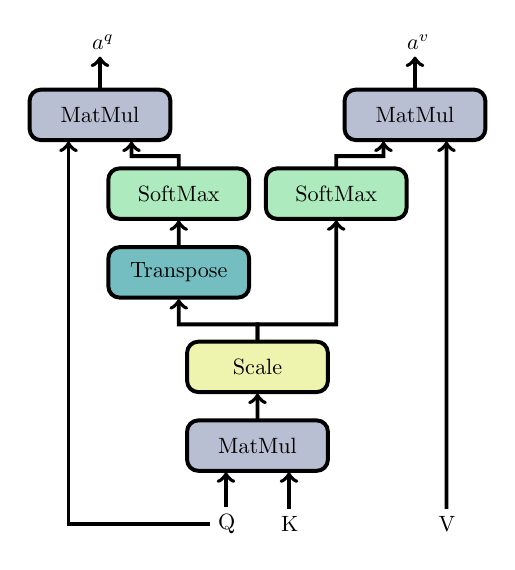
\begin{tikzpicture}[scale=0.8, every node/.style={scale=.8}]
\tikzstyle{sqr} = [rectangle, rounded corners, minimum width=2cm, text width=2cm, minimum height=.8cm,text centered, draw=black, line width=.5mm]
\tikzstyle{rect} = [rectangle, rounded corners, minimum width=1cm, minimum height=2cm,text centered, draw=black, line width=.5mm]

\node (mm1) [sqr, fill=pastelblue!40] {MatMul};
\node (scale) [sqr, fill=pastellyellow, above of=mm1, yshift=.25cm] {Scale};
\node (trans) [sqr, fill=pastellblue, above of=scale, yshift=.5cm, xshift=-1.25cm] {Transpose};
\node (sm1) [sqr, fill=pastellgreen, above of=trans, yshift=.25cm] {SoftMax};
\node (sm2) [sqr, fill=pastellgreen, right of=sm1, xshift=1.5cm] {SoftMax};
\node (mm2) [sqr, fill=pastelblue!40, above of=sm1, yshift=.25cm, xshift=-1.25cm] {MatMul};
\node (mm3) [sqr, fill=pastelblue!40, above of=sm2, yshift=.25cm, xshift=1.25cm] {MatMul};

\node (Q) [text width=.25cm, below of=mm1, yshift=-.25cm, xshift=-.5cm] {Q};
\node (K) [text width=.25cm, below of=mm1, yshift=-.25cm, xshift=.5cm] {K};
\node (V) [text width=.25cm, below of=mm1, yshift=-.25cm, xshift=3.cm] {V};


\draw[->, line width=.5mm] (mm1) -- (scale);
\draw[->, line width=.5mm] (scale.north) |- +(-1.25cm, .25cm) -- (trans.south);
\draw[->, line width=.5mm] (scale.north) |- +(1.25cm, .25cm) -- (sm2.south);
\draw[->, line width=.5mm] (trans) -- (sm1);
\draw[->, line width=.5mm] (sm1.north) |- +(-.75cm, .17cm) -- ($(mm2.south) + (.5cm, 0)$);
\draw[->, line width=.5mm] (sm2.north) |- +(.75cm, .17cm) -- ($(mm3.south) + (-.5cm, 0)$);

\draw[->, line width=.5mm] (Q) -- ($(mm1.south) + (-.5cm, 0)$);
\draw[->, line width=.5mm] (K) -- ($(mm1.south) + (.5cm, 0)$);
\draw[->, line width=.5mm] (V) -- ($(mm3.south) + (.5cm, 0)$);
\draw[->, line width=.5mm] (Q) -| ($(mm2.south) + (-.5cm, 0)$);

\draw[->, line width=.5mm] (mm2.north) -- +(0, .5cm);
\draw[->, line width=.5mm] (mm3.north) -- +(0, .5cm);

\node (aq) [text width=.25cm, above of=mm2, yshift=.15cm, xshift=0cm] {$a^q$};
\node (av) [text width=.25cm, above of=mm3, yshift=.15cm, xshift=0cm] {$a^v$};

\end{tikzpicture}

\end{document}